\chapter{Introdução}

Veículos aéreos não tripulados (VANTs) são aeronaves equipadas com sistemas embarcados, sensores e atuadores que permitem a realização de voos autônomos ou remotamente controlados. Eles são comumente classificados em dois grupos: veículos de asas rotativas, como helicópteros e quadrotores, e veículos de asas fixas, como aviões. 

Há diversas aplicações para VANTs, alguns exemplos são:

\begin{itemize}
	\itemsep0em
	\item Pulverização de culturas;
	\item Condução de rebanhos;
	\item Monitoramento de estradas;
	\item Inspeção da linhas de energia;
	\item Entrega de suprimentos em locais de difícil acesso.
	\end{itemize}
	
O simulador apresentado neste manual está associado ao ProVANT\footnote{provant.eng.ufmg.br}. O ProVANT consiste em uma parceria entre a Universidade Federal de Santa Catarina e a Universidade Federal de Minas Gerais, com o objetivo de realizar pesquisas e desenvolver novas tecnologias para aperfeiçoar o desempenho de VANTs. Neste contexto, atualmente, o ProVANT está focado no desenvolvimento de VANTs Tilt-rotor.  O Tilt-rotor é uma aeronave que possui configuração híbrida, portanto apresenta as principais vantagens das aeronaves de asa fixa e de asa rotativa, como por exemplo consumo reduzido de energia em voos de cruzeiro e decolagem e pouso na vertical. Ele pode operar tanto em ambientes fechados quanto abertos.

Atualmente o ProVANT possui três tipos de linhas de projeto:
	\begin{enumerate}
		\item Mecânico/Aerodinâmico;
		\item Instrumentação/Eletrônica;
		\item Projeto de estratégias de controle e estimação de estados;
	\end{enumerate}

O projeto Mecânico/Aerodinâmico já conta com 5 versões de VANTs que foram nomeadas como VANT 1.0, 2.0, 2.1, 3.0 e 4.0, as Figuras \ref{vant1}, \ref{vant2}, \ref{vant21}, \ref{vant3} e \ref{vant4} ilustram, respectivamente, essas versões. A Instrumentação/Eletrônica está em estágio avançados, com todos os circuitos eletrônicos desenvolvidos e realizando melhorias nos mesmos. Com relação ao Projeto de estratégias de controle e estimação de estados, no contexto do projeto diversas estratégias de controle foram propostas por alunos de mestrado e doutorado.

Ainda com relação ao Projeto de estratégias de controle e estimação de estados, alguns trabalhos científicos foram desenvolvidos. Em \cite{Donadel2015} controladores baseados nas técnicas \textit{Linear Quadratic Regulator} (LQR), $\mathcal{H}_\infty$ linear e $\mathcal{H}_2/\mathcal{H}_\infty$ linear misto foram desenvolvidos para o VANT 1.0. Com o objetivo de rastreamento de trajetória. Alguns destes controladores foram validados através de voos experimentais. Em \cite{Marcelinol2014} é apresentado uma técnica de controle não-linear baseado em \textit{feedback linearization} com o objetivo de transporte de carga para o VANT 2.0, ainda com o mesmo objetivo, \cite{Richard2016} apresenta o desenvolvimento de um controlador baseado na técnica \textit{Model Preditive Control} (MPC). Em \cite{Brenner2016}, trabalhou-se com o transporte de carga do VANT 2.0, no entanto, abordou-se o problema de seguimento de trajetória do ponto de vista da carga, para o qual foram projetados estimadores de estados robustos. Em \cite{Daniel2016}, desenvolveu-se uma estratégia de controle adaptativo com a finalidade de seguimento de trajetória para o VANT 3.0. 
		
\begin{figure} [H]
		\centering
		\begin{minipage}{.5\textwidth}
			\centering
			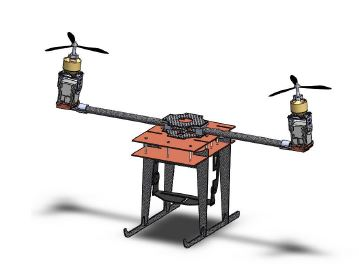
\includegraphics[height=3.5cm]{figuras/VANT1}
			\caption{Projeto mecânico VANT 1.0.}
			\label{vant1}
		\end{minipage}%
		\begin{minipage}{.5\textwidth}
			\centering
			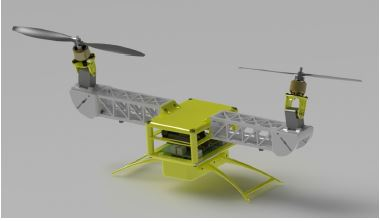
\includegraphics[height=3.5cm]{figuras/VANT2}
			\caption{Projeto mecânico VANT 2.0.}
			\label{vant2}
			\end{minipage}
	\end{figure}
					
	\begin{figure} [H]
		\centering
		\begin{minipage}{.5\textwidth}
			\centering
			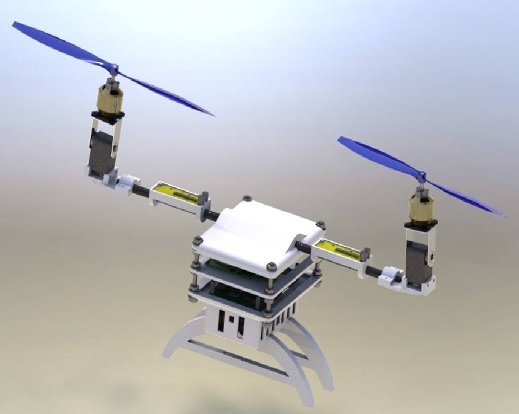
\includegraphics[height=3.5cm]{figuras/VANT21}
			\caption{Projeto mecânico VANT 2.1.}
			\label{vant21}
		\end{minipage}%
		\begin{minipage}{.5\textwidth}
			\centering
			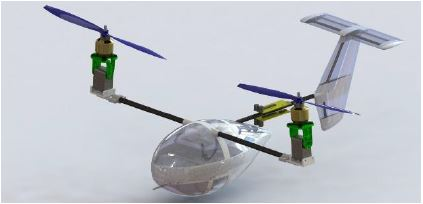
\includegraphics[height=3.5cm]{figuras/VANT3}
			\caption{Projeto mecânico VANT 3.0.}
			\label{vant3}
		\end{minipage}
	\end{figure}
								
	\begin{figure} [H]
		\centering
		\begin{minipage}{.5\textwidth}
			\centering
			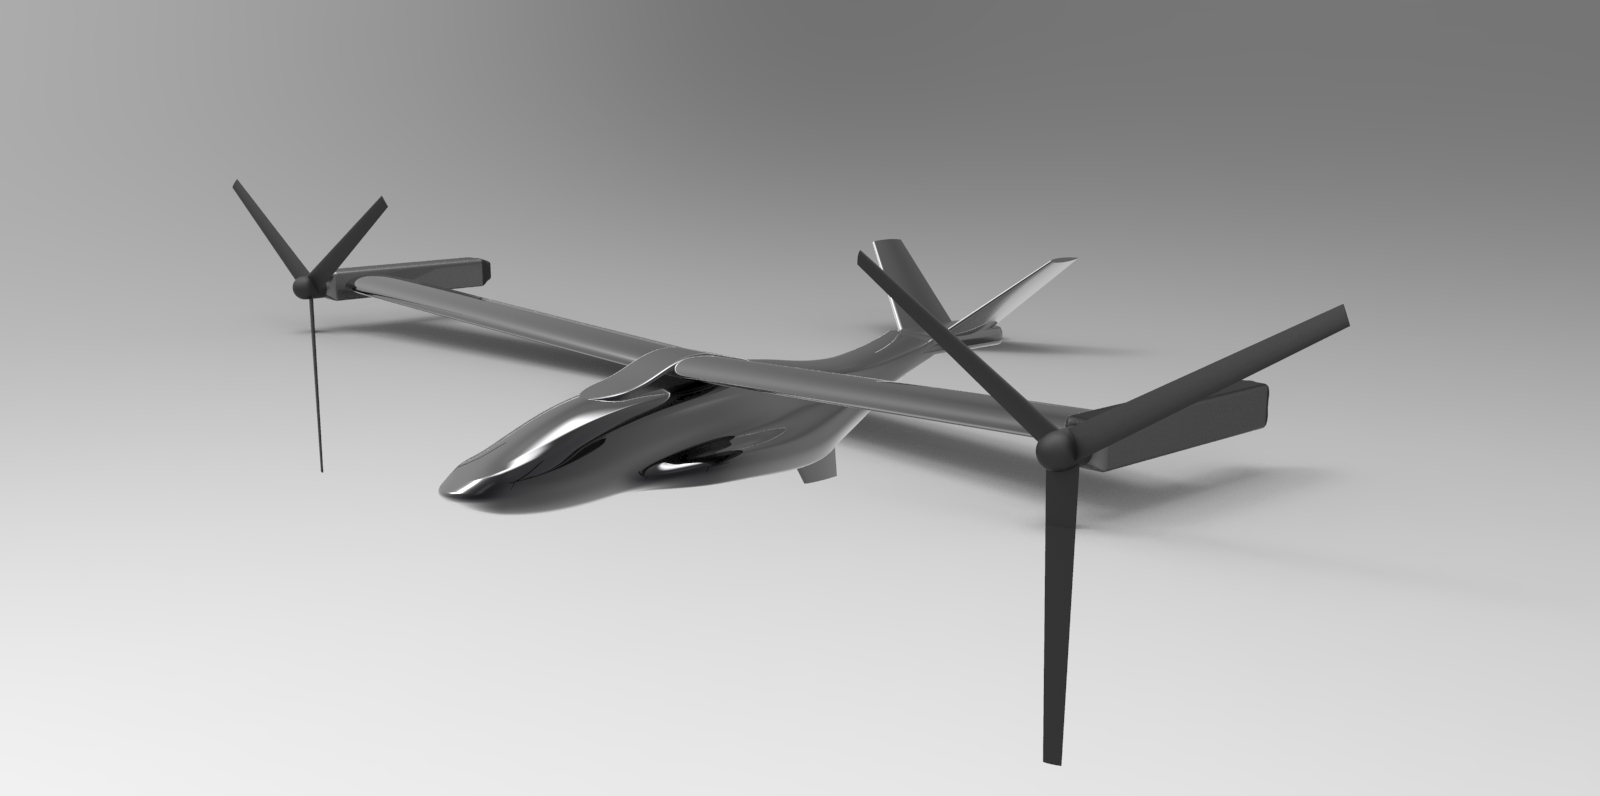
\includegraphics[height=3.5cm]{figuras/VANT4}
			\caption{Projeto mecânico VANT 4.0.}
			\label{vant4}
		\end{minipage}
	\end{figure}

O simulador ProVANT tem o objetivo de ser uma ferramenta confiável e de fácil utilização. O intuito é possibilitar a redução de custos e de tempo necessário para o projeto e validação de estratégias de controle.